\documentclass[tikz]{standalone}

\usepackage{tikz}
\usetikzlibrary{quotes}
%\usepackage{}
%\use...library{}

%\tikzset{every figure} = []
\begin{document}
	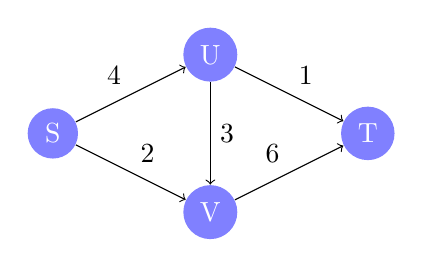
\begin{tikzpicture} 
		%\node (nom node) at(x,y) [options separées par virgules] {affichage} ;
		\node (node 1) at(0, 1) [circle,double, double distance =1.2pt,text=white,fill=blue!50,] {S} ;
		\node (node 2) at(2, 0) [circle,double, double distance =1.2pt,text=white,fill=blue!50,] {V} ;
		\node (node 3) at(2, 2) [circle,double, double distance =1.2pt,text=white,fill=blue!50,] {U} ;
		\node (node 4) at(4, 1) [circle,double, double distance =1.2pt,text=white,fill=blue!50,] {T} ;
		
%(nom node): charactères interdits: ( ) [ ] ; { } ,
%at(x,y): optionel : x et y doivent être des coordonnées viables: des nombres 
%[options séparées par virgules]:  les options du nœud. En détail certain: 			 
	%fill=couleur
	%label=texte du label ou label={texte du label} ou label={:texte du label}
	%label={position du label:texte du label}
	%label={[couleur du label]:texte du label}
	%label={[couleur du label]position du label:texte du label}
	%texte du label : charactères interdits: ; { } ,
	%draw ou draw=
	%draw=couleur{Affichage}: charactères interdits: { } [ ]; 
	
		%\path (nom node A) edge[options separées par virgules] (nom node B);
		\path 
		(node 1) edge[->,"2"] (node 2)
		(node 1) edge[->,"4"] (node 3)
		(node 3) edge[->,"3"] (node 2)
		(node 3) edge[->,"1"] (node 4)
		(node 2) edge[->,"6"] (node 4)
		;

%nom node: fait reference à un nom de nœud défini plus haut
%[options séparées par virgules]:  les options de l’arrête/arc. En détail certain:
	%-> ou <-ou -: le sens de l’arrête
	%"edge_label": indication sur l’arrête, pour Dijkstra indique le poids, pour Dijkstra option obligatoire 
	% edge_label : charactères interdits: ; , 
	%color=couleur: la couleur de l’arrete.
	\end{tikzpicture}
\end{document}
